%
% tikztemplate.tex -- template for standalon tikz images
%
% (c) 2021 Prof Dr Andreas Müller, OST Ostschweizer Fachhochschule
%
\documentclass[tikz]{standalone}
\usepackage{amsmath}
\usepackage{times}
\usepackage{txfonts}
\usepackage{pgfplots}
\usepackage{csvsimple}
\usetikzlibrary{arrows,intersections,math}
\begin{document}
\def\skala{1}
\begin{tikzpicture}[>=latex,thick,scale=\skala]

% add image content here

\begin{scope}[xshift=-3.6cm]
%\clip (-3.3,-3) rectangle (3.3,3);
\node at (0,0) {
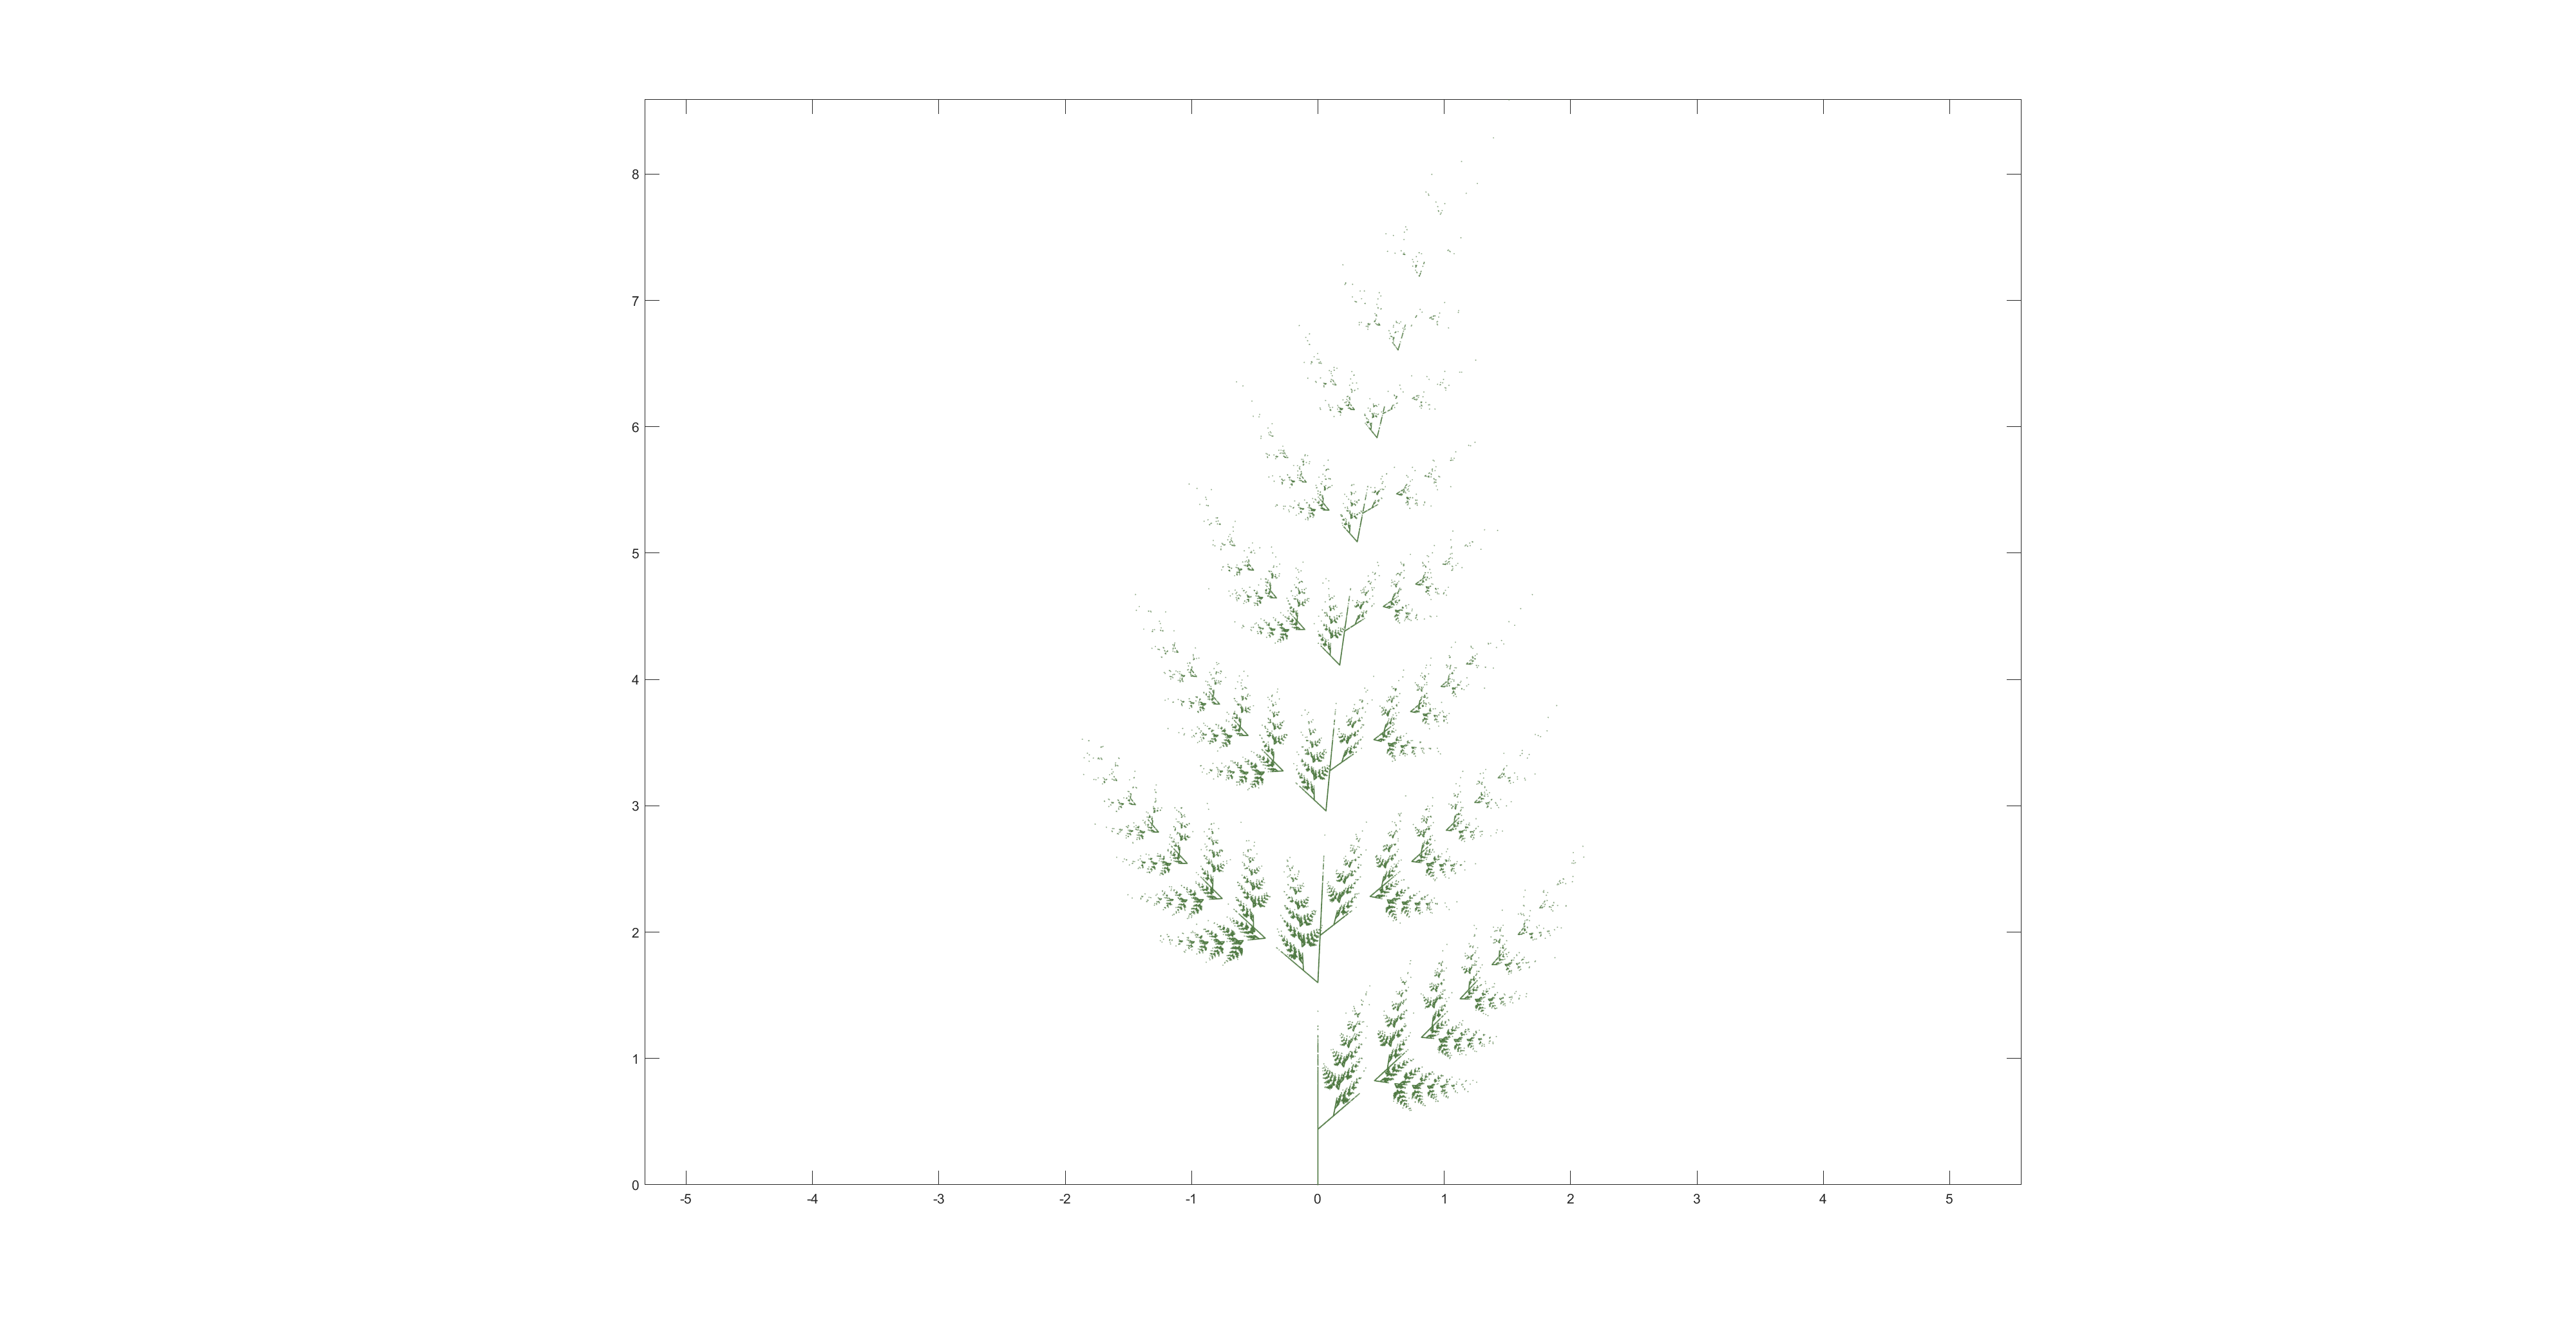
\includegraphics[width=6.8cm]{farnnotweight-eps-converted-to.pdf}
};
\node at (0.2,-5.7) {(a)};
\end{scope}

\begin{scope}[xshift=3.6cm]
%\clip (-3.3,-3) rectangle (3.3,3);
\node at (0,0) {
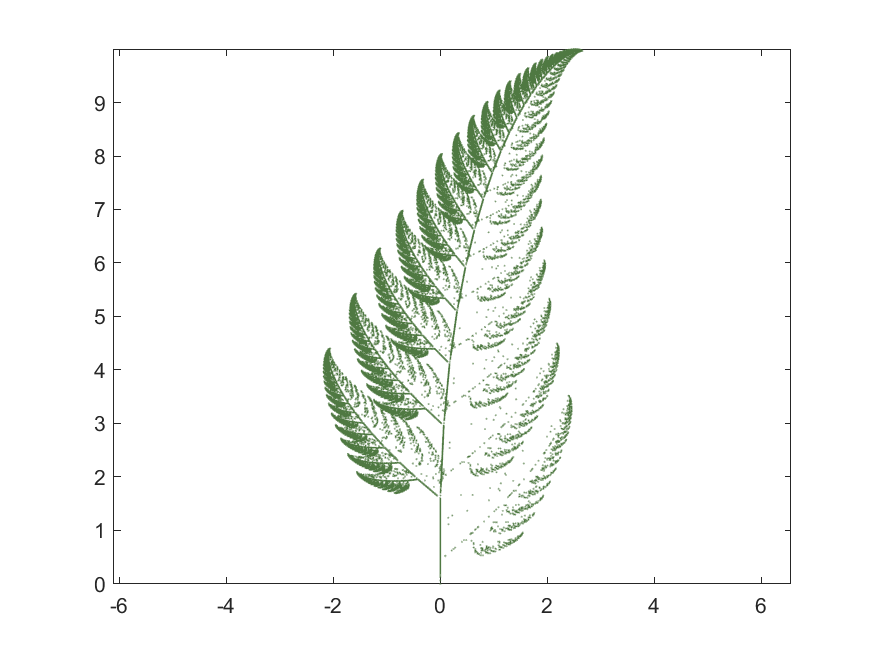
\includegraphics[width=6.8cm]{farnrightwight-eps-converted-to.pdf}
};
\node at (0.2,-5.7) {(b)};
\end{scope}

\end{tikzpicture}
\end{document}

